\section{Результаты измерений}
\subsection{Определение ширины щели}

$\lambda = 532\;\text{нм}$

$a_{1} = 4{,}3 \pm 0{,}5 \; \text{см}$, $b_{1} = 120{,}5 \pm 0{,}5 \;\text{см}$, $\Gamma = b_{1} / a_{1} = 28 \pm 3$.

\[
    \Gamma = b_{1} / a_{1} = 28 \pm 3
\]


\begin{tabular}{|l|l|}
\hline
$b,\;\text{мм}$ & $D_1,\;\text{мм}$\\\hline
$\left(50 \pm 5\right)\cdot 10^{-3}$ & $2{,}0 \pm 0{,}3$\\\hline
$\left(100 \pm 5\right)\cdot 10^{-3}$ & $3{,}0 \pm 0{,}3$\\\hline
$\left(150 \pm 5\right)\cdot 10^{-3}$ & $4{,}0 \pm 0{,}3$\\\hline
$\left(200 \pm 5\right)\cdot 10^{-3}$ & $5{,}5 \pm 0{,}3$\\\hline
$\left(250 \pm 5\right)\cdot 10^{-3}$ & $6{,}0 \pm 0{,}3$\\\hline
$\left(300 \pm 5\right)\cdot 10^{-3}$ & $7{,}0 \pm 0{,}3$\\\hline
$\left(350 \pm 5\right)\cdot 10^{-3}$ & $8{,}0 \pm 0{,}3$\\\hline
$\left(400 \pm 5\right)\cdot 10^{-3}$ & $9{,}0 \pm 0{,}3$\\\hline
$\left(450 \pm 5\right)\cdot 10^{-3}$ & $11{,}0 \pm 0{,}3$\\\hline
$\left(500 \pm 5\right)\cdot 10^{-3}$ & $12{,}0 \pm 0{,}3$\\\hline
\end{tabular}

\begin{figure}[ht!]
    \center{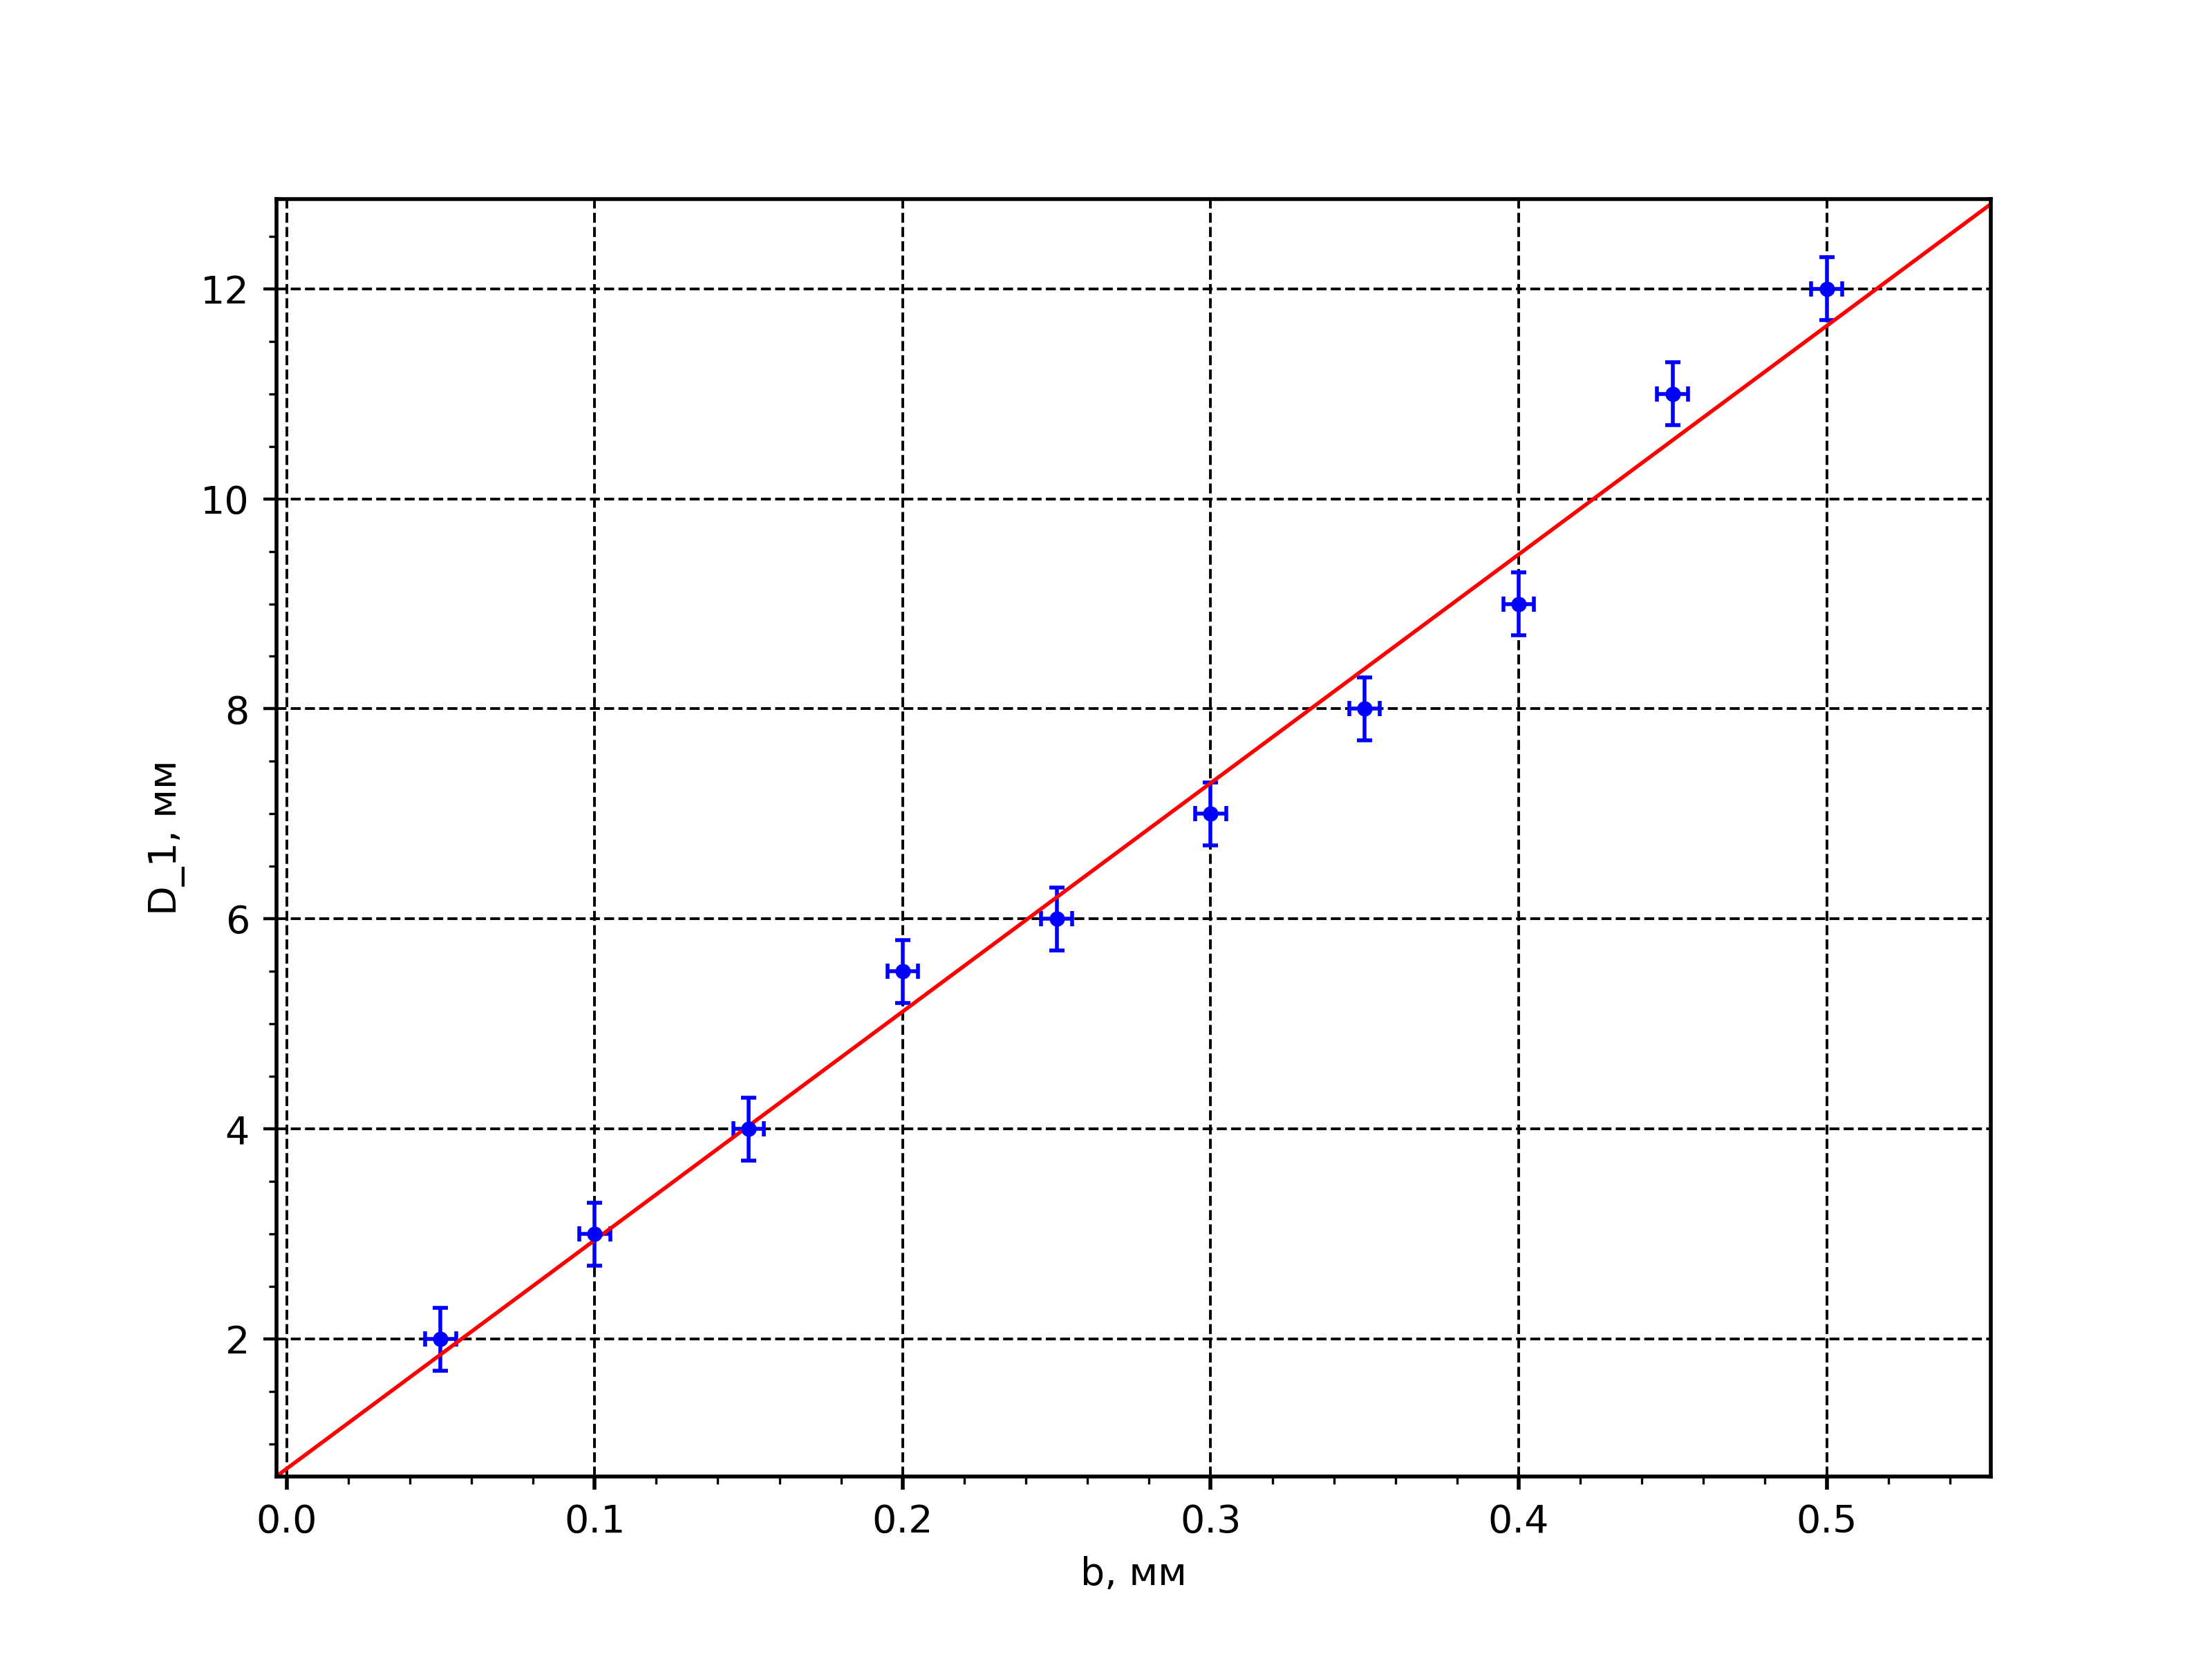
\includegraphics[width=0.8\linewidth]{../img/p1.png}}
\end{figure}

\[
\Gamma = 23 \pm 2
\]

\begin{figure}[ht!]
    \center{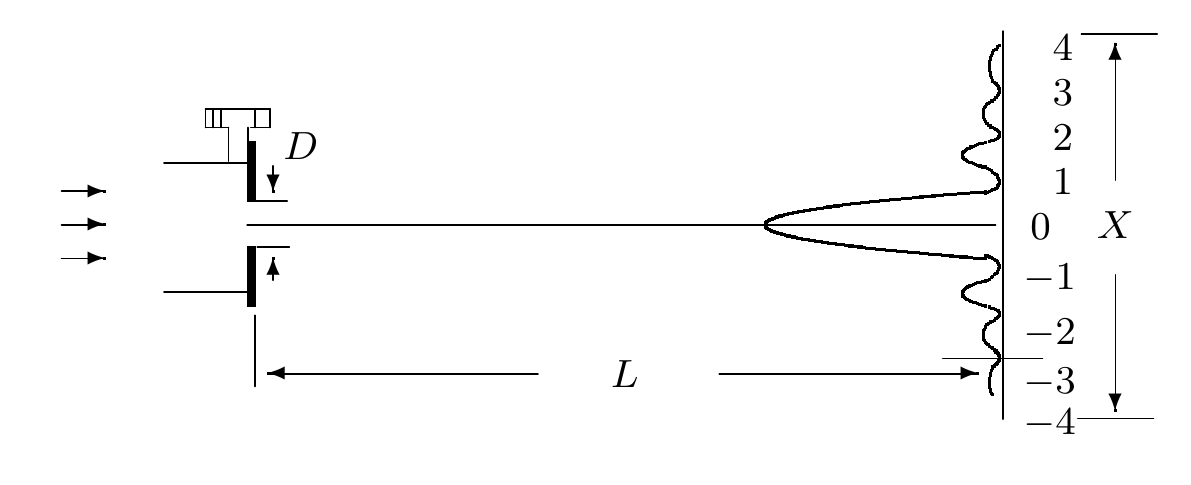
\includegraphics[width=0.8\linewidth]{../img/ris2.png}}
\end{figure}

\[
    X = \frac{\lambda}{d_{c}}L
\]

$L = 127{,}0 \pm 0{,}5 \;\text{см}$

\begin{tabular}{|l|l|l|}
\hline
$b,\;\text{мм}$ & $X,\;\text{мм}$ & $b_c,\;\text{мм}$\\\hline
$\left(100 \pm 5\right)\cdot 10^{-3}$ & $7{,}01 \pm 0{,}05$ & $\left(964 \pm 8\right)\cdot 10^{-4}$\\\hline
$\left(150 \pm 5\right)\cdot 10^{-3}$ & $4{,}75 \pm 0{,}05$ & $\left(142 \pm 2\right)\cdot 10^{-3}$\\\hline
$\left(200 \pm 5\right)\cdot 10^{-3}$ & $3{,}28 \pm 0{,}05$ & $\left(206 \pm 3\right)\cdot 10^{-3}$\\\hline
$\left(250 \pm 5\right)\cdot 10^{-3}$ & $2{,}72 \pm 0{,}05$ & $\left(248 \pm 5\right)\cdot 10^{-3}$\\\hline
$\left(300 \pm 5\right)\cdot 10^{-3}$ & $2{,}36 \pm 0{,}05$ & $\left(286 \pm 6\right)\cdot 10^{-3}$\\\hline
$\left(350 \pm 5\right)\cdot 10^{-3}$ & $1{,}95 \pm 0{,}05$ & $\left(346 \pm 9\right)\cdot 10^{-3}$\\\hline
$\left(400 \pm 5\right)\cdot 10^{-3}$ & $1{,}69 \pm 0{,}05$ & $0{,}40 \pm 0{,}012$\\\hline
$\left(450 \pm 5\right)\cdot 10^{-3}$ & $1{,}47 \pm 0{,}05$ & $0{,}46 \pm 0{,}02$\\\hline
\end{tabular}

\begin{figure}[ht!]
    \center{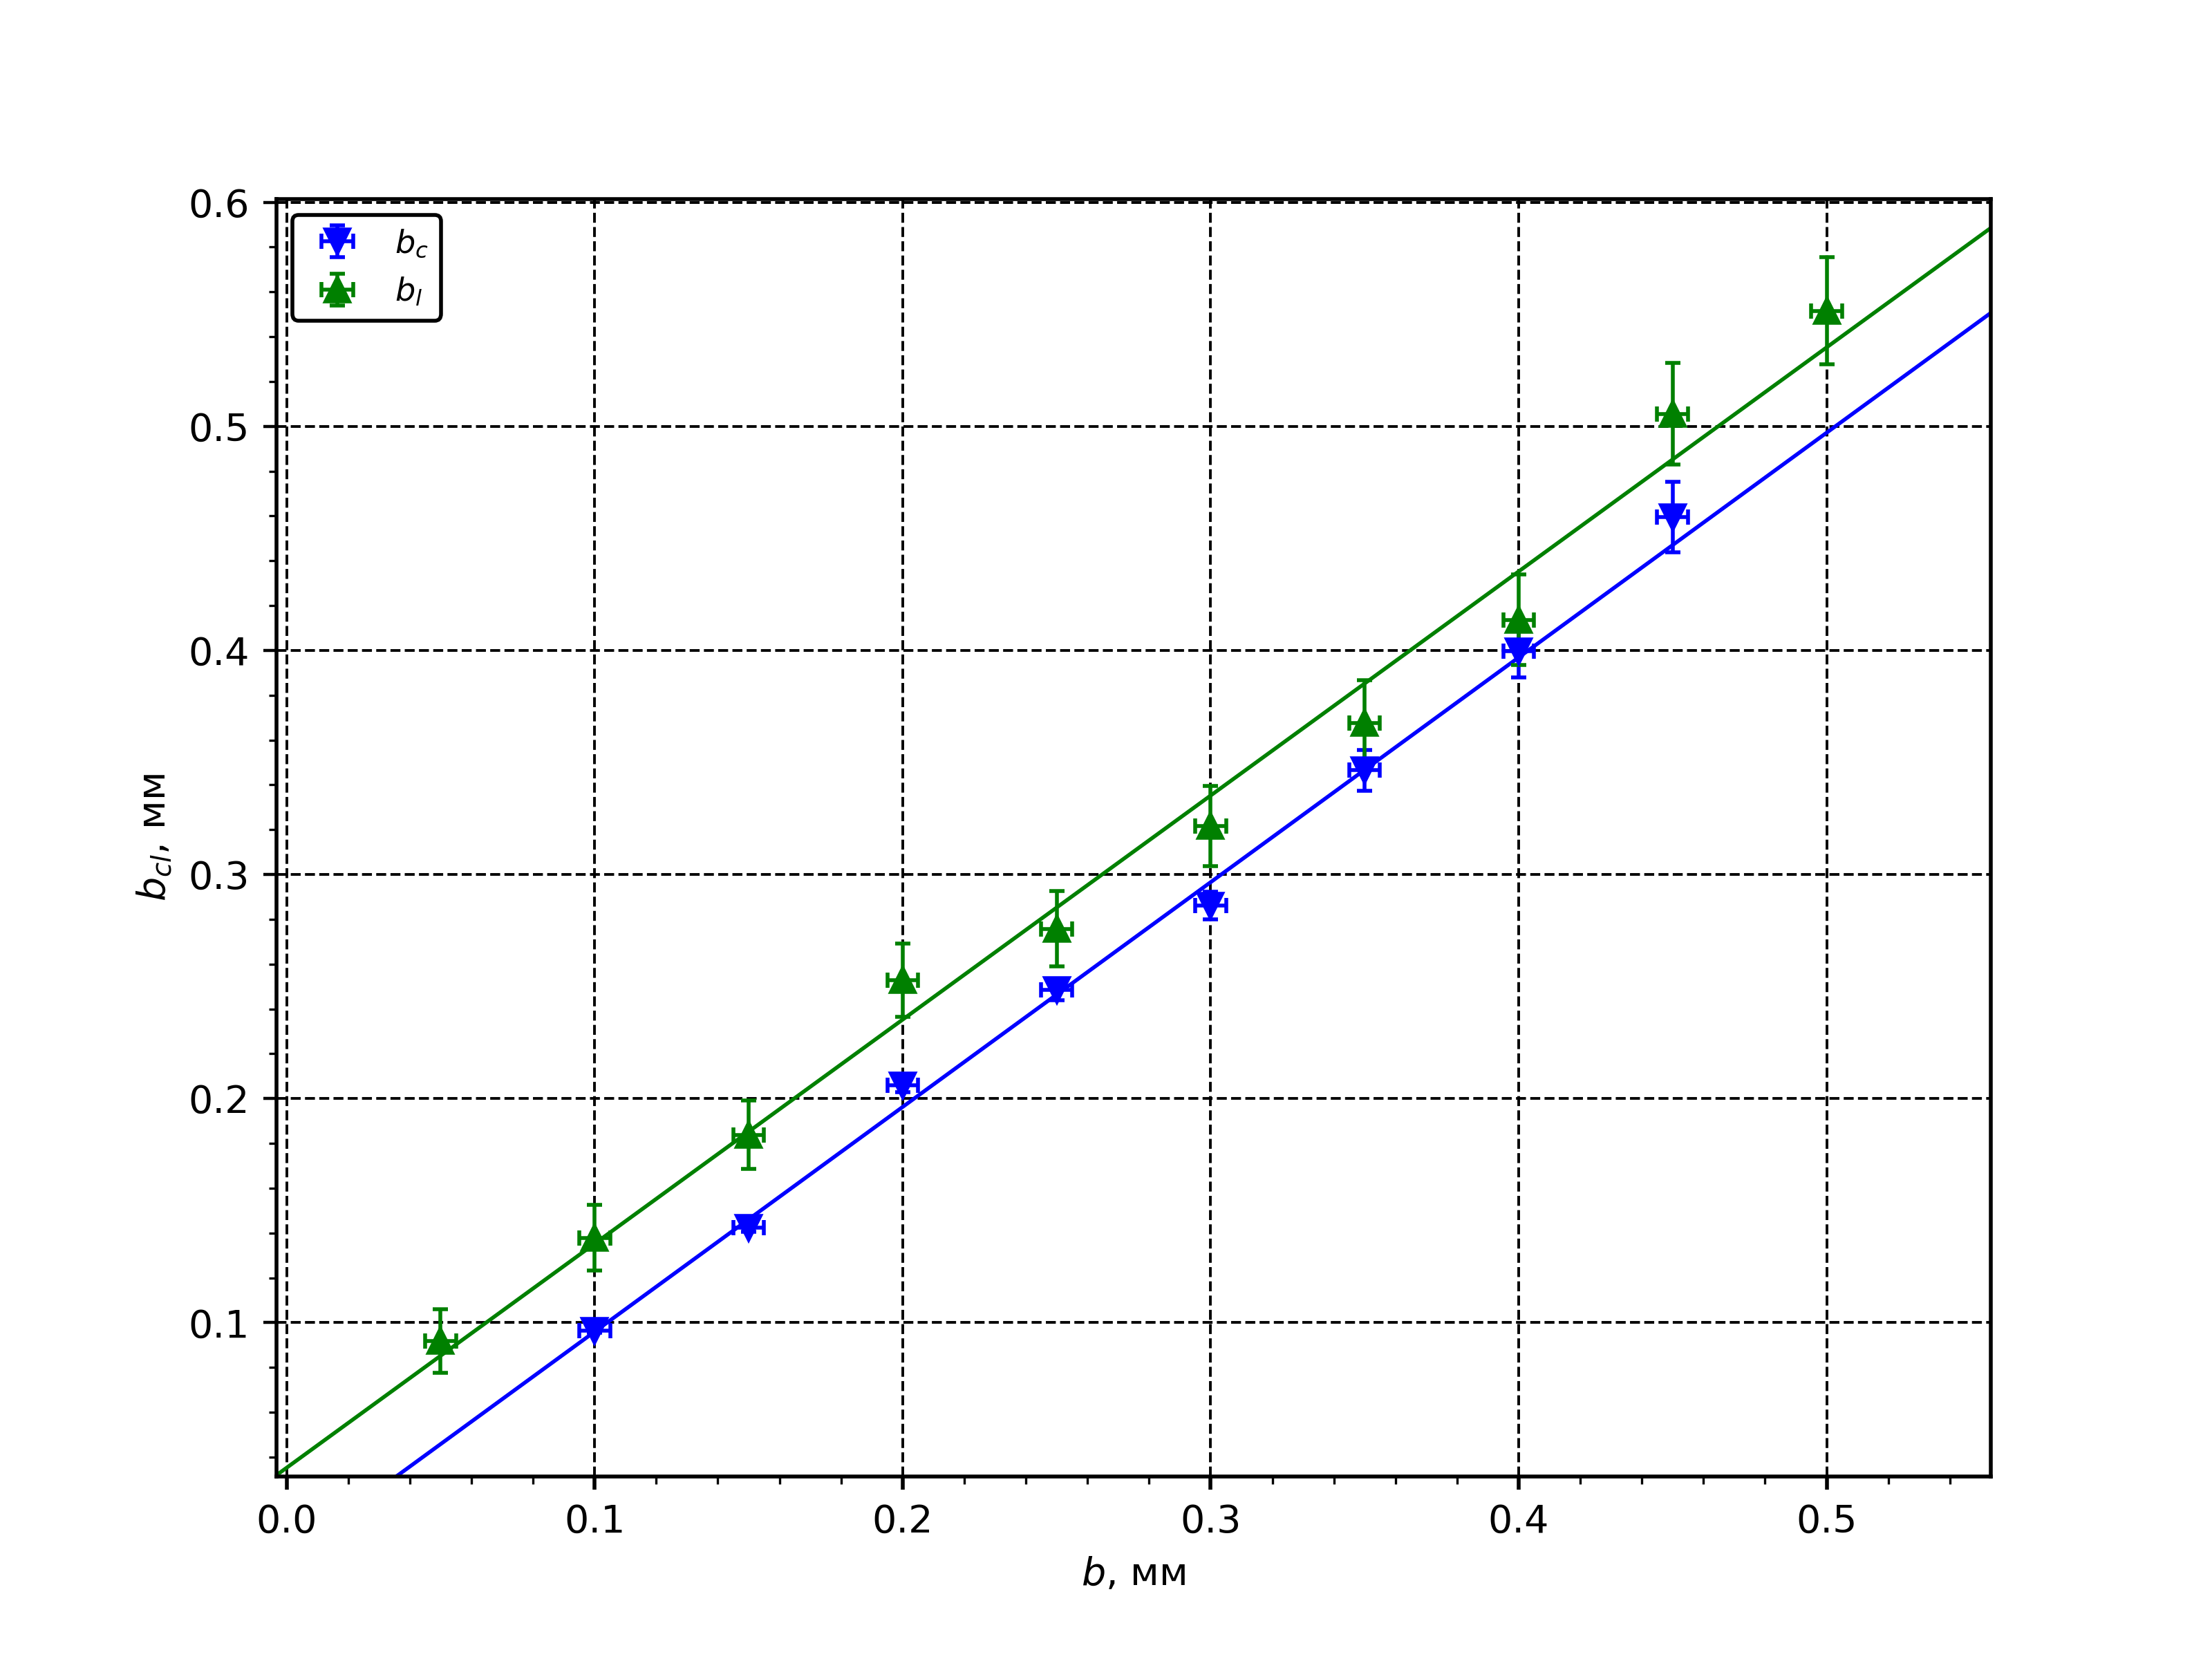
\includegraphics[width=0.8\linewidth]{../img/p2.png}}
\end{figure}

\subsection{Определение периода решеток}
\[
    \Delta X = \frac{X}{2m} = \frac{ \lambda}{d_{c}}L
\]

\begin{tabular}{|l|l|l|l|}
\hline
номер сетки & $X, \;\text{мм}$ & $m$ & $d_{c}, \;\text{мкм}$ \\\hline
    1, низ & $122 \pm 0{,}5$ & 2 & $11{,}5 \pm 0{,}1$ \\\hline
    1, верх & $122 \pm 0{,}5$ & 2 & $11{,}5 \pm 0{,}1$ \\\hline
    2, низ & $124 \pm 0{,}5$ & 5 & $28{,}4 \pm 0{,}2$ \\\hline
    2, верх & $124 \pm 0{,}5$ & 5 & $28{,}4 \pm 0{,}2$ \\\hline
    3, низ & $60 \pm 0{,}5$ & 5 & $58{,}0 \pm 0{,}1$ \\\hline
    3, верх & $60 \pm 0{,}5$ & 5 & $58{,}0 \pm 0{,}1$ \\\hline
\end{tabular}

Картины от верхних и нижних сеток одинаковы, поэтому измерения будут проводиться только для нижних.

\begin{figure}[ht!]
    \center{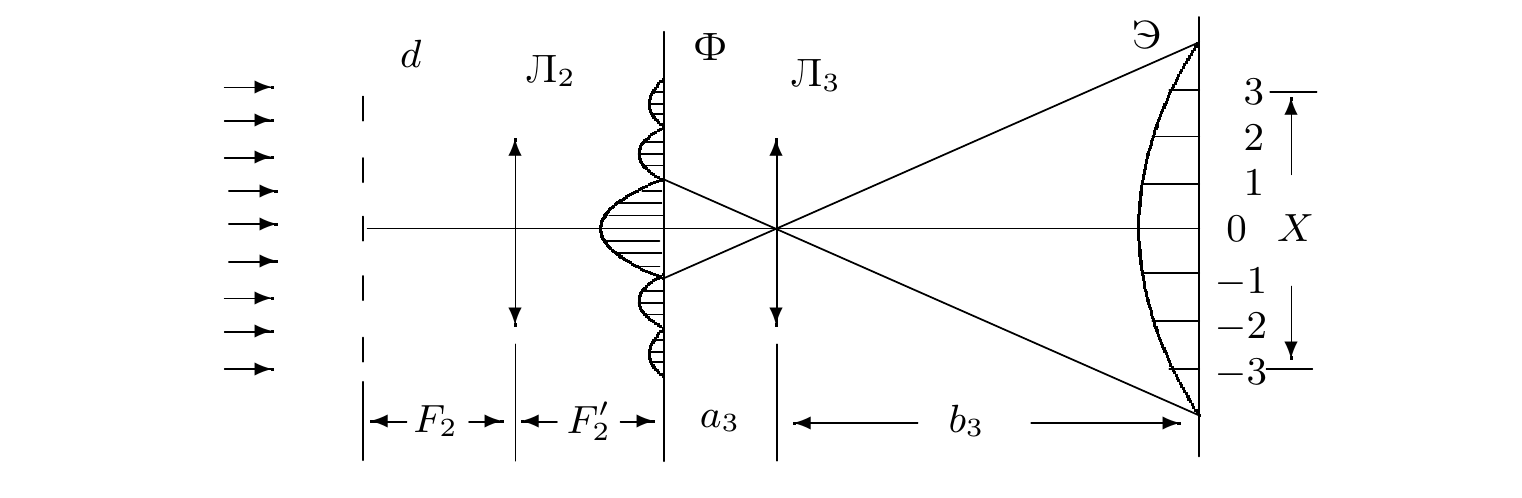
\includegraphics[width=0.8\linewidth]{../img/ris3.png}}
\end{figure}

$F_{2} = 110\;\text{мм}$, $F_{3} = 25\;\text{мм}$

\begin{tabular}{|l|l|l|l|}
\hline
    номер сетки & $X,\;\text{мм}$ & $m$ & $d_{l}, \;\text{мкм}$ \\\hline
    1 & $341 \pm 0{,}5$ & 1 & $11{,}1 \pm 2{,}2$ \\\hline
    2 & $257 \pm 0{,}5$ & 2 & $29{,}5 \pm 3{,}1$ \\\hline
    3 & $180 \pm 0{,}5$ & 3 & $63{,}3 \pm 4{,}4$ \\\hline
\end{tabular}

$\Gamma_{3} = 3{,}5 \pm 0{,}5$

\subsection{Мультиплицирование}
\begin{figure}[ht!]
    \center{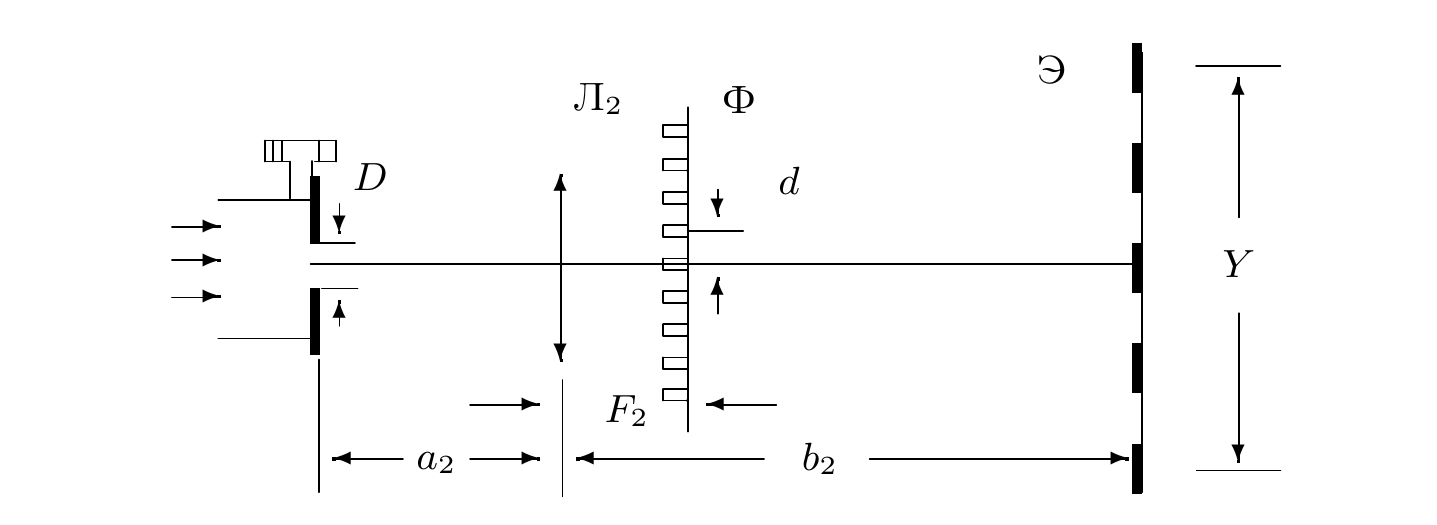
\includegraphics[width=0.8\linewidth]{../img/fig4.png}}
\end{figure}

$\Delta y = \Delta y / \Gamma$, $\Gamma = 10$, $\Delta \Gamma / K$.

\begin{tabular}{|l|l|l|l|l|}
\hline
    номер сетки & $Y,\;\text{мм}$ & $K$ & $\Delta Y,\;\text{мм}$ & $\Delta y,\;\text{мм}$ \\\hline
    1 & $119 \pm 0{,}5$ & 2 & $59{,}5 \pm 0{,}3$ & $5{,}7 \pm 0{,}1$ \\\hline
    2 & $118 \pm 0{,}5$ & 5 & $23{,}6 \pm 0{,}1$ & $2{,}3 \pm 0{,}1$ \\\hline
    3 & $70 \pm 0{,}5$ & 6 & $11{,}7 \pm 0{,}1$ & $1{,}3 \pm 0{,}1$ \\\hline
\end{tabular}

\begin{figure}[ht!]
    \center{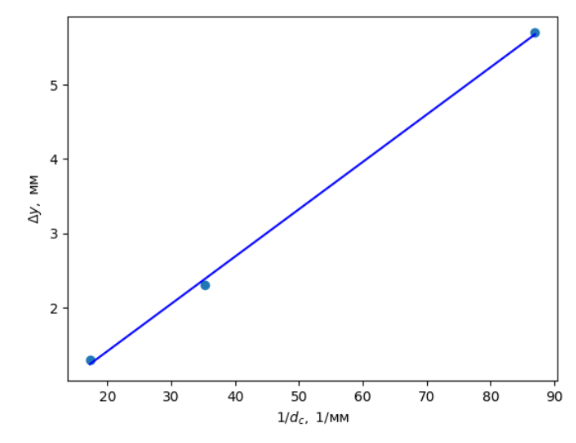
\includegraphics[width=0.8\linewidth]{../img/ris7.png}}
\end{figure}


